\scanpage{61}
plus des $\deleted{\widetilde\Pi_\omega}\Pi_\omega$ et $\deleted{\widetilde\Pi_i},\Pi_i$, des régions
\[
\widetilde\Sigma_r=\widetilde\Sigma_{\deleted{\unsure{r}}i\deleted{\unsure{\omega}}}^{\omega,\varepsilon}
\]
associés aux repères $r=(i,\omega,\deleted{\unsure{\bar\omega|\varpi}}\varepsilon)$ de $(J,\uline{\varepsilon})$ (ou ce qui revient au $=$, de $(J,\uline{\unsure{\bar\omega|\varpi}})$), qu'on peut identifier, géométriquement, aux \inserted{douze} triangles-drapeaux, \inserted{$D_r=P_\varepsilon Q_iR_{\omega i}$} correspondants à la subdivision barycentrique standard de la carte dans $\Sigma$ définie par l'équateur $\Sigma_{\mathbb R}$ et par les trois points $R_i$ sur celui-ci.
\figure{
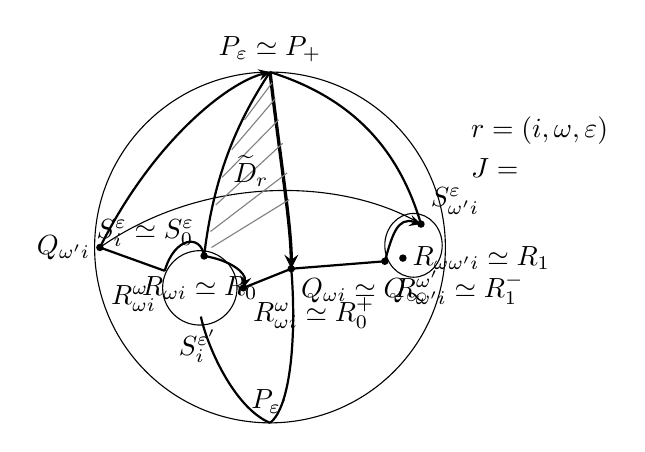
\begin{tikzpicture}[scale=1.35,>=stealth]
\coordinate (N) at(0,1.65);\coordinate (S)at(0,-1.65);\coordinate (L)at(-1.6,0);\coordinate (Q)at(.2,-.2);\coordinate (T)at(1.25,-.1);\coordinate (A)at(-.62,-.08);\coordinate (B)at(-.25,-.38);\coordinate (C)at(1.08,-.13);\coordinate (D)at(1.42,.22);
\draw[thin] (0,0)circle(1.65);
\draw[thin] (L) .. controls(-.6,.7)and(.7,.65)..(D);
\draw[->,thick] (L)..controls(-1.1,1.0)and(-.4,1.55)..(N);
\draw[thick] (N)..controls(.8,1.4)and(1.22,.9)..(D);
\draw[thick] (N)..controls(-.4,1.05)and(-.55,.5)..(A);
\draw[->,very thick] (N)..controls(.1,.8)and(.2,.2)..(Q);
\draw[thick] (Q)..controls(.25,-.8)and(.2,-1.5)..(S);
\draw[thick] (S)..controls(-.35,-1.5)and(-.6,-.9)..(-.65,-.65);
\draw[thick] (L)--(-.99,-.22);\draw[thick] (B)--(Q)--(C);
\draw[->,thick] (-.99,-.22)..controls(-.9,.1)and(-.65,.13)..(A)..controls(-.37,-.12)and(-.22,-.24)..(B);
\draw[thin] (-.66,-.38)circle(.35);
\draw[->,thick] (C)..controls(1.15,.12)and(1.2,.29)..(D);
\draw[thin] (1.35,.02)ellipse(.27 and .3);
\foreach \a/\b/\c/\d in {-.56/.15/.16/.7,-.51/.4/.12/.98,-.45/.66/.08/1.2,-.36/.92/.05/1.4,-.24/1.2/.02/1.55,-.55/.0/.18/.45}{\draw[thin,gray](\a,\b)--(\c,\d);}
\node at(-.18,.72){$\widetilde D_r$};
\node[above] at(N){$P_\varepsilon\simeq P_+$};\node[above]at(S){$P_{\varepsilon'}$};
\node[left]at(L){$Q_{\omega'i}$};\node[below right]at(Q){$Q_{\deleted{\unsure{\omega}}i}\simeq Q_\infty$};
\node[above left]at(A){$S_i^\varepsilon\simeq S_0^\varepsilon$};\node[below]at(-.68,-.68){$S_i^{\varepsilon'}$};
\node[below left]at(-.98,-.2){$R_{\unsure{\omega i}}^{\omega'}$};
\node[below right]at(B){$R_{\unsure{\omega i}}^\omega\simeq R_0^+$};
\node at(-.66,-.38){$R_{\deleted{\unsure{\omega}}i}\simeq\deleted{\unsure{R_0}}$};
\node[below right]at(C){$R_{\omega'i}^{\omega'}\simeq R_1^-$};
\node[above right]at(D){$S_{\omega'i}^\varepsilon$};
\node[right]at(T){$R_{\deleted{\unsure{\omega}}\omega'i}\simeq R_1$};
\node[right]at(1.8,1.1){$r=(i,\omega,\varepsilon)$};\node[right]at(1.8,.75){$J=$};
\fill(L)circle(1pt);\fill(Q)circle(1pt);\fill(A)circle(1pt);\fill(B)circle(1pt);\fill(C)circle(1pt);\fill(D)circle(1pt);\fill(T)circle(1pt);
\end{tikzpicture}}
Le ``\unsure{tronc|vrai}'' \inserted{sur $\widetilde\Sigma$} au sens évident d'un tel triangle est un quadrilatère $\widetilde D_r$
\[
P_\varepsilon Q_{\omega'i}R_i^\omega S_i^\varepsilon\simeq P_+Q_\infty R_0^+S_0^+.
\]
On aura à travailler, au ``voisinage\unsure{''|``} immédiat'' de ces \deleted{repères} \inserted{drapeaux} \deleted{\unsure{triangles des}} $\widetilde\Sigma_r$, avec les symétriques de $\Sigma_r$ p.r. à ses trois côtés, et \unsure{se trouve sur|par suite sur} $\widetilde\Sigma$, \deleted{\unsure{pour ce qui}} ce qui conduit à regarder la réunion de $\Sigma_r$ avec ses trois frères
\[
\tau(\Sigma_r),\widetilde\sigma_i(\Sigma_r),\widetilde\sigma_{\omega i}(\Sigma_r)
\]
(qui \inserted{resp.} correspondent, sur la sphère standard avec le repère correspondant au triangle $P_+Q_\infty R_0$, à $\tau,\widetilde\sigma_\infty,\widetilde\sigma_0$) et sur $\widetilde\Sigma$ à prendre
\[
(41)\qquad\widetilde\Sigma_r=\widetilde\Sigma_i^{\omega,\varepsilon}=\widetilde D_r\cup\tau(\widetilde D_r)\cup\widetilde\sigma_i(\widetilde D_r)\cup\widetilde\sigma_{\omega i}(\unsure{\Sigma_+|\Sigma_r})
\]
limités par le contour
\[
P_\varepsilon Q_{\omega'i}R_{\omega i}^{\omega'}S_i^{\unsure{\varepsilon|\varepsilon'}}R_{\omega i}^{\omega}S_i^{\varepsilon'}P_{\varepsilon'}Q_iR_{\omega'i}^{\omega'}S_{\omega'i}^\varepsilon P_\varepsilon
\]
\margin{60}
